\documentclass{ccg-topic}

\institution{University of Colorado}
\coursenum{MATH/APPM 1300/1350}
\coursename{Calculus 1}
\semester{Spring 2019}
\topic{Theorems for Final Review}
\author{Colton Grainger}
\date{\today}
\email{colton.grainger@colorado.edu}
\thanks{I am freely quoting Pete L. Clark's \emph{Honors Calculus} and Micheal Spivak's \emph{Calculus}.}

\begin{document}
\frontstuff

\section{Interval theorems}

Here, we'll state two so-called \textbf{Interval Theorems}, which concern an arbitrary continuous function defined on a closed, bounded interval.

\begin{thm}[Intermediate Value Theorem]
    \label{thm:intermediate_value_theorem}
    Let $f \colon \bkt{a,b} \to \R$ be a continuous function defined on a closed, bounded interval. Suppose that $f(a) < 0$ and $f(b) > 0$. Then there exists $a < c < b$ such that $f(c) = 0$.
\end{thm}

\begin{thm}[Extreme Value Theorem]
    \label{thm:extreme_value_theorem}
    Let $f \colon [a,b] \to \R$ be a continuous function defined on a closed, bounded interval. Then $f$ is bounded and assumes its maximum and minimum values: there are real numbers $m_{\mathrm{min}}$ and $M_{\mathrm{max}}$ such that
    \begin{enumerate}
        \item For all $x$ between $a \le x \le b$, the function value $f(x)$ is between $m_{\mathrm{min}} \le f(x) \le M_{\mathrm{max}}$.
        \item There is at least one $x_{\mathrm{min}}$ between $a \le x_{\mathrm{min}} \le b$ such that $f(x_{\mathrm{min}}) = m_{\mathrm{min}}$.
        \item There is at least one $x_{\mathrm{max}}$ between $a \le x_{\mathrm{max}} \le b$ such that $f(x_{\mathrm{max}}) = M_{\mathrm{max}}$.
    \end{enumerate}
\end{thm}

Now we'll give three examples of the IVT and the EVT ``at work''. First for the IVT.

\begin{ex}[The Möbius strip is not orientable]
    \label{ex:the_mobius_strip_is_unorientable}
    The surface $[0,2\pi] \times [-1,1]$ mapped into $\R^3$ with ends identified by a $180^\circ$ rotation is called a \term{Möbius strip}.

    \begin{figure}[htpb]
        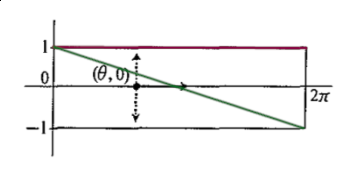
\includegraphics[width=0.55\linewidth]{images/moebius-unwound.png}
        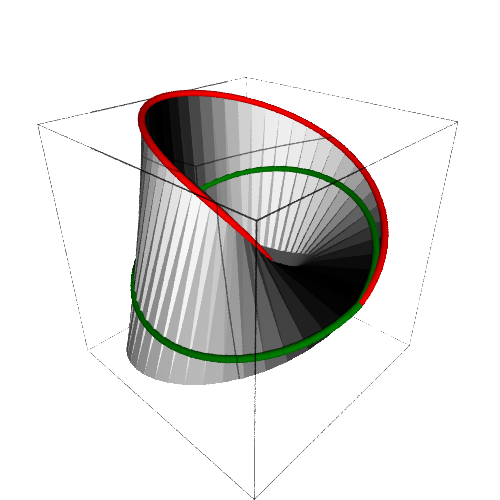
\includegraphics[width=0.3\linewidth]{images/moebius.png}
        \caption{The surface $[0, 2\pi]\times (-1,1)$ and a Möbius strip constructed from it.}
        \label{fig:images/moebius-unwound}
    \end{figure}
    Fact: a continuous function $f \colon [0, 2\pi] \to [-1,1]$ can be graphed on the Möbius strip if and only if $f(0) = -f(2\pi)$. (For example, $\cos(2\cdot 0) = - \cos (2\cdot 2\pi)$, so $f(\theta) = \cos(2\theta)$ can be graphed on the Möbius strip.) Suppose that $f \colon [0, 2\pi] \to [-1,1]$ is continuous and \emph{can} be graphed on the Möbius strip. Because $f(0) = - f(2\pi)$, by the Intermediate Value Theorem, there exists an angle $c$ that lies between $0 < c < 2\pi$ and for which $f(c) = 0$. 
   
    In \emph{differential geometry}, this conclusion shows that the Möbius strip is \emph{not orientable}, as in, it is a surface where we cannot choose a ``\emph{right hand rule}'' (one of your fingers would have to disappear!).
\end{ex}

Now for the EVT. Here's an edge case to consider (which is one of the reasons that we don't ``do calculus over $\Q$'', that is, why we don't only work with functions whose domains are \emph{rational numbers}).

\begin{ex}[The Extreme Value Theorem fails over $\Q$.]
    \label{ex:the_extreme_value_theorem_fails_over_q_}
    Recall from way back: the natural numbers $\N$ are the counting numbers $0, 1, 2, 3, \ldots$, the integers $\Z$ are formed by taking all the natural numbers and all the negative natural numbers, and the rational numbers $\Q$ are formed by taking fractions of the form $m/n$, where $m$ and $n$ are integers, and $n \neq 0$. The set of real numbers $\R$ is formed by \emph{completing} the rational numbers with respect to convergent sequences. For example, the number $\sqrt{2} \in \R$ can be written as the \emph{limit} of a sequence of rational numbers 
    \[\sqrt{2} = 1.4142135623731\ldots\] 
    but is \emph{not} itself a rational number.

    Now, ``consider the function $f \colon [0, 2]_{\Q}$ given by $f(x) = \frac{1}{x^2 - 2}$. This function is well defined for \emph{all} points of $[0,2]_{\Q}$, because $\sqrt{2}$ is not a rational number (why?). It is also a continuous function. However, it is \emph{not bounded above}. By taking rational numbers close to $\sqrt{2}$, the denominator $x^2 - 2$ becomes arbitrarily small, and thus $f(x)$ becomes arbitrarily large. So $f$ does not attain a maximum value. Thus the Extreme Value Theorem fails over $\Q$.''
    \begin{figure}[htpb]
        \centering
        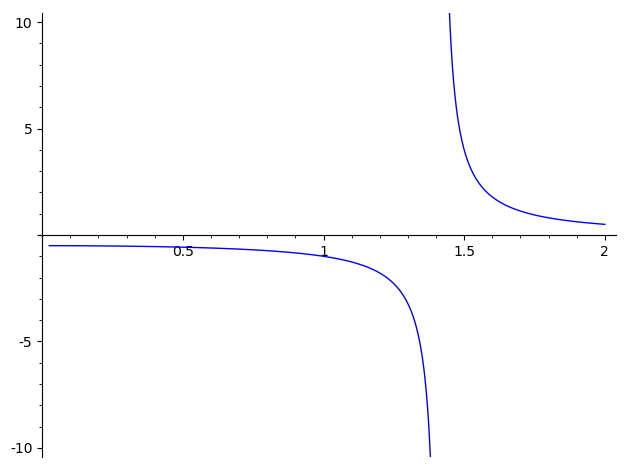
\includegraphics[width=0.6\linewidth]{images/2019-05-05-poles.png}
        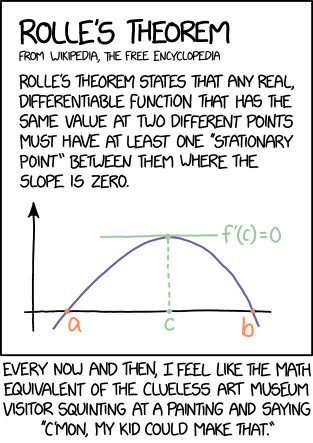
\includegraphics[width=0.3\linewidth]{images/2019-05-05-rolles.png}
        \caption{$f(x) = \frac{1}{x^2 - 2}$ is continuous on $[0,2]_\Q$; also Rolle's theorem.}
        \label{fig:images/2019-05-05-poles}
    \end{figure}
\end{ex}

\begin{ex}[Rolle's theorem]
    \label{ex:rolle_s_theorem}
    In fact, the extreme value theorem allows us to prove to \emph{Mean Value Theorem}. A relatively simple special case of the mean value theorem is the \emph{Rolle's Theorem}, which states: 
    \emph{If $f \colon \bkt{a,b} \to \R$ is continuous on $\bkt{a,b}$, and if $f$ is differentiable on $(a,b)$, and if $f(a) = f(b)$, then there exists $c$ stricly between $a < c < b$ such that $f'(c) = 0$.}
\end{ex}

\section{Axiomatic integration}
``As you probably know, the general idea is to construe $\int_a^b f$ as the result of some kind of limiting process, wherein we divide $[a,b]$ into subintervals and take the sum of the areas of certain rectangles which approximate the function $f$ at various points of the interval (\textrm{Riemann sums}). But wait! Before plunging into the details of this limit process, let's take a more \textrm{axiomatic} approach.'' 

The following properties of the definite integral should \emph{feel} like \emph{conservation laws}:%
    \footnote{%
    For example, one physical interpretation of $\int_c^c f = 0$ would be to consider a \emph{Carnot cycle} for a classical thermodynamical engine.
    }

    \begin{defn}[Axioms for integrable functions]
        \label{defn:axioms_for_integrable_functions}
        For any integrable function(s) of the form $f \colon [a,b] \to \R$:
        \begin{enumerate}
            \item If $f = C$ is a constant function, then $\int_a^b C = C(b-a)$.
            \item If $f(x) \le g(x)$ for all $x$ between $a \le x \le b$, then $\int_a^b f \le \int_a^b g$.
            \item If $a \le c \le b$, then $\int_a^b f = \int_a^c f + \int_c^b f$.
        \end{enumerate}
    \end{defn}

\begin{todo}[Closed loops in the real line]
    \label{todo:closed_loops_in_the_real_line}
    Show that $\int_a^b f = \int_a^c f + \int_c^b f$ implies $\int_c^c f = 0$ for any $f \colon [a,b] \to \R$ and any $c$ between $a \le c \le b$. 
\end{todo}

``It turns out that these three axioms imply many of the other properties we want an integral to have. Even more, there is essentially only one way to define $\int_a^b f$ to satisfy the axioms. But, in case this business seems abstruse, then on the first pass just imagine the that the set of integrable functions is just the set of all continuous functions $f \colon [a,b] \to \R$.''  We are justified in taking ``integrable'' to mean ``continuous'' because of the following theorem:

\begin{thm}[Continuity on a closed, bounded interval implies integrability]
    \label{thm:sufficient_condition_for_integrability}
    Let $f \colon \bkt{a,b} \to \R$ be a continuous function defined on a closed, bounded interval. Then $f$ is integrable: $\int_a^b f$ exists, and satisfies the axioms, and is finite.
\end{thm}

Pretty quickly from the axioms, one can prove:

\begin{thm}[Fundamental Theorem of Calculus]
    \label{thm:fundamental_theorem_of_calculus}
    Let $f \colon [a,b] \to \R$ be any integrable function. For all points $x$ between $a \le x \le b$, define $\mathcal{F}(x) = \int_a^x f(t)\dd{t}$. Then \hfill
    \begin{enumerate}
        \item  The function $\mathcal{F} \colon [a,b] \to \R$ is continuous at every point $c$ between $a \le c \le b$.
        \item If $f$ is continuous at a point $c$, then $\mathcal{F}$ is differentiable at $c$, and $\mathcal{F}'(c) = f(c)$.
        \item If $f$ is continuous and $F$ is any antiderivative of $f$, (i.e., a function $F \colon \bkt{a,b} \to \R$ such that $F'(x) = f(x)$ for all $x \in \bkt{a,b}$) then $\int_a^b f = F(b) - F(a)$.
    \end{enumerate}
\end{thm}

\begin{todo}[Differentiating the definite integral]
    \label{todo:differentiating_the_definite_integral}
    Prove that if $h$ is continuous, $f$ and $g$ are differentiable, and 
    \begin{equation*}
        F(x) = \int_{f(x)}^{g(x)}h(t)\dd{t} 
    \end{equation*}
    then $F'(x) = h(g(x))\cdot g'(x) - h(f(x)) \cdot f'(x)$. (Hint: split into two cases you know how to handle.)
\end{todo}

\begin{todo}[Definite integrals of periodic functions]
    \label{todo:definite_integrals_of_periodic_functions}
    A function $f$ is \textrm{periodic}, with \textrm{period} $a$ if $f(x + a) = f(x)$ for all $x$.
    \begin{enumerate}
        \item If $f$ is periodic with period $a$, and integrable on $[0,a]$, show that $\int_0^a f = \int_b^{b+a} f$ for all $b$.
        \item Find a function $f$ such that $f$ is not periodic, but $f'$ is. (Hint: choose a periodic $g$ for which it can be guaranteed that $f(x) = \int_0^x g$ is not periodic.
    \end{enumerate}
\end{todo}

Having shown results straight from the axioms, it's time to bring out the Riemann sums and show that such a definite integral actually exists, and can actually be computed. Since it's tedious, I'll skip the definition of the definite integral as a limit Riemann sums, in order to have time to state a rather cute fact:

\begin{fact}[Preview of the Darboux integral]
    \label{fact:}
    For any continuous (as in, integrable) function $f \colon [0,1] \to \R$, we have 
    \[
        \lim_{n \to \infty} \frac{1}{n} \sum\limits_{k=1}^{n} f\paren{ \frac{k}{n} } = \int_0^1 f(x) \dd{x}.
    \]
\end{fact}

\begin{ex}[Arctangent as a sum]
    \label{ex:arctangent_as_a_sum}
    Consider the limit 
    \begin{equation*}
        \lim_{n \to \infty} \sum\limits_{k=1}^{n} \frac{n}{k^2 + n^2} = \lim_{n \to \infty} \frac{1}{n} \sum\limits_{k=1}^{n} \frac{n^2}{k^2 + n^2} = \lim_{n \to \infty} \frac{1}{n} \sum\limits_{k=1}^{n} \frac{1}{\paren{\frac{k}{n}}^2 + 1} = \lim_{n \to \infty} \frac{1}{n}\sum\limits_{k=1}^{n} f \paren{\frac{k}{n}}
    \end{equation*}
    where $f(x) = \frac{1}{x^2 + 1} $. Thus the limit is
    \begin{equation*}
        \int_0^1 \frac{\dd{x}}{x^2 + 1} = \arctan 1 - \arctan 0 = \frac{\pi}{2}.
    \end{equation*}
\end{ex}
\end{document}
